% Talk at Howard University on 2022-08-31

\documentclass{beamer} % "sans" is text default 

\usetheme{metropolis}
\usefonttheme{professionalfonts}
\usepackage{arev}

\usepackage[justification=centering]{caption}
\usepackage[labelfont=tiny, textfont=tiny]{subcaption}
\usepackage{fontenc}

\usepackage{amsmath}

\usepackage{tcolorbox}

\usepackage{dcolumn}
\usepackage{booktabs}
\usepackage{threeparttable}

\definecolor{SU_red}{HTML}{AA0000}          % Header/footer backgroup

\setbeamercolor{frametitle}{bg=SU_red}
\setbeamercolor{title separator}{fg=SU_red}
\setbeamercolor{progress bar in section page}{fg=SU_red}

\title{Impact of COVID-19 Lockdowns on Hunger, Labor Market Outcomes, and Household Coping Mechanisms: Evidence from Uganda}
\date{31 August 2022}
\author{
Shamma A. Alam
\and
Claus C. P\"ortner
\and
Ishraq Ahmed
}
\institute{Albers School of Business and Economics, Seattle University \and Center for Studies in Demography and Ecology, University of Washington}

\begin{document}
\graphicspath{{../figures/}}
\DeclareGraphicsExtensions{.eps,.jpg,.pdf,.mps,.png}


\maketitle

\section{Introduction}

\begin{frame}{Main Question}

\begin{tcolorbox}
How did Covid lockdowns affect food insecurity? 
\end{tcolorbox}

\end{frame}


\begin{frame}{Why Interesting?}


Welfare effects

\bigskip

Understand Uganda's long-term development prospects

\bigskip

Exogenous systematic shock (as opposed to idiosyncratic) 


\end{frame}


\begin{frame}{Among Strictest Lockdowns in Sub-Saharan Africa}

\begin{figure}
\centering
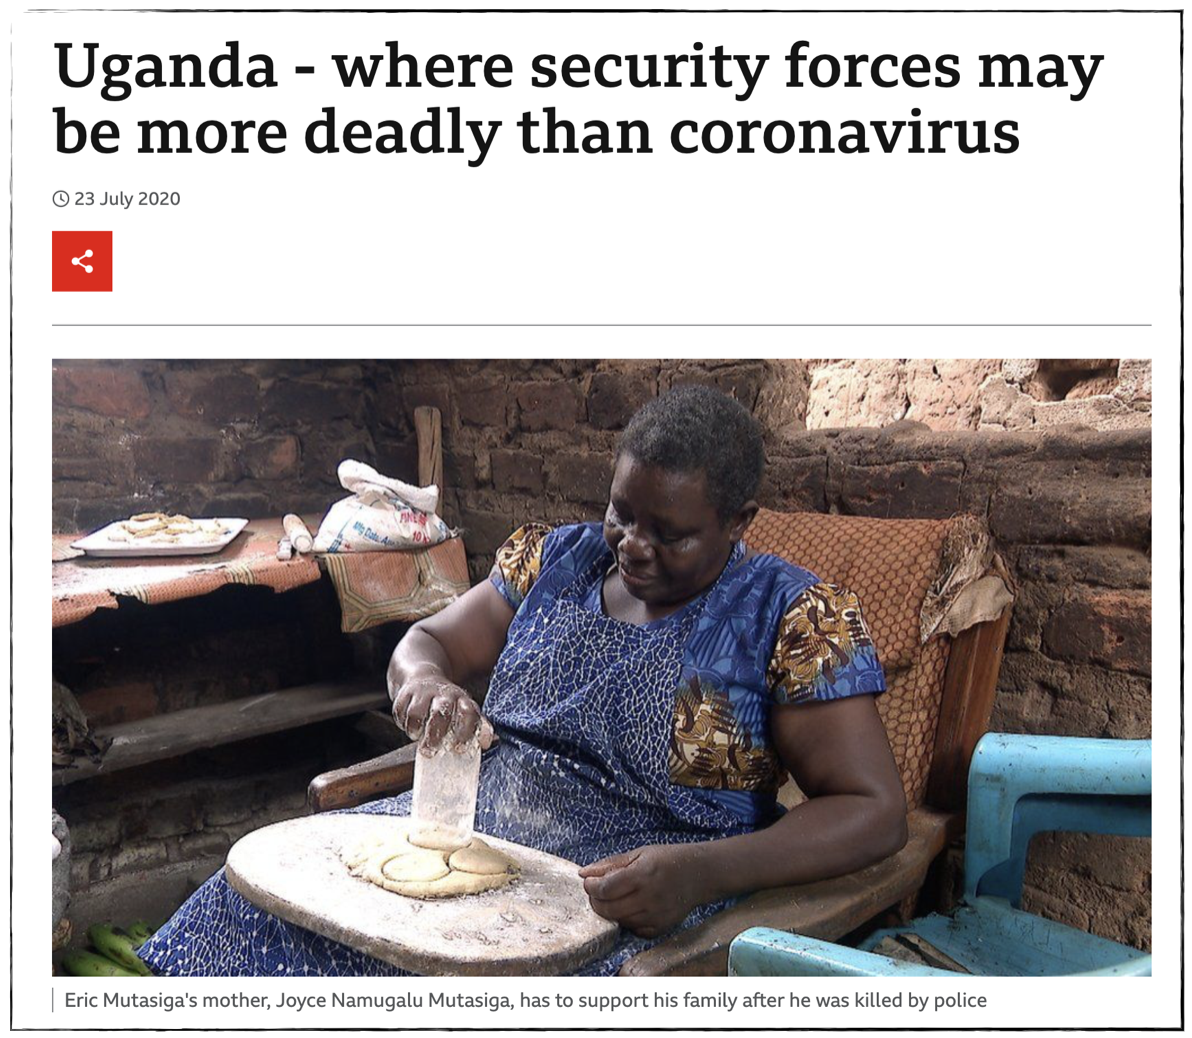
\includegraphics[width=0.8\textwidth, keepaspectratio]{bbc-headline.png}
\end{figure}


\end{frame}


\begin{frame}{1st Covid Lockdowns in Uganda}


\begin{itemize}
\item 18 March 2020: travel restrictions, cancellation 
of public gatherings 
\item 30 March 2020: total lockdown with curfew; no public/private transport; 
all non-essential businesses closed
\item June 2020: resumption of public transport and opening of businesses
\end{itemize}

\end{frame}

\begin{frame}{2nd Covid Lockdowns in Uganda}

\begin{itemize}
\item 18 June 2021: total lockdown with curfew; no public/private transport;
banning of public gatherings; closure of schools, open-market shutdowns
\item 2 August 2021: partial lifting of restrictions; still curfew and 
no public gatherings or school; 
\item Mid-September 2021: further lifting of restrictions
\end{itemize}

\end{frame}



\section{Estimation Strategy and Data}

\begin{frame}{Estimation Strategy}

Linear Fixed effects on longitudinal data (household/individual)

\bigskip

Identification: Temporal variation in lockdowns, $L_t$

\begin{multline}
Y_{i,t} = \beta_0 + \beta_1 L_t + \sum_{r} \beta_{2r}  Round_r  \\
+ \beta_3 Cases_{i,t} + \beta_4 Size_{i,t-1}  + \delta_i + \epsilon_{i,t}
\end{multline}

\end{frame}

\begin{frame}{Uganda High-Frequency Phone Survey}

Aim: understand effects of Covid

\bigskip

Sampling: Uganda National Panel Survey 2019/20 households

\bigskip

Sample size: 2,227 (3,098 households in 2019/20 survey)


\end{frame}


\begin{frame}{Survey Timing}

Rounds:
\begin{itemize}
\item 1: June 2020 --- Lockdown
\item 2: August 2020
\item 3: September 2020
\item 4: October 2020
\item 5: February 2021
\item 6: March 2021
\item 7: October 2021 --- Lockdown
\end{itemize}

\end{frame}


\section{Food Insecurity}

\begin{frame}{Lockdowns Significant Increases Food Insecurity}

\begin{center}
\begin{tabular}{@{} l D{.}{.}{2.6}  D{.}{.}{1.3} @{}}
\toprule
Outcome variables:	& \multicolumn{1}{c}{Lockdown} & \multicolumn{1}{c}{Mean}   \\ \midrule
Any food insecurity	&  0.238^{\textrm{***}}	&  0.593 \\ 	
					& (0.011)	& \\
\bottomrule
\end{tabular}
\end{center}

\end{frame}

\begin{frame}{Aspects of Food Insecurity -- 1}

\begin{center}
\begin{tabular}{@{} l D{.}{.}{2.6}  D{.}{.}{1.3} @{}}
\toprule
Outcome variables:	& \multicolumn{1}{c}{Lockdown} & \multicolumn{1}{c}{Mean}   \\ \midrule
Worry about not enough food & 0.303^{\textrm{***}} &  	0.405 \\
 & (0.012)	& \\
Lack healthy and nutritious food	& 0.218^{\textrm{***}} &  	0.486 \\
&(0.012) & \\
Only a few kinds of food to eat	& 	0.211^{\textrm{***}} &	0.468 \\
&(0.012) & 	\\
Had to skip a meal & 	0.212^{\textrm{***}} &	0.224 \\
&(0.010) & 	\\
\bottomrule
\end{tabular}
\end{center}

\end{frame}



\begin{frame}{Aspects of Food Insecurity -- 2}

\begin{center}
\begin{tabular}{@{} l D{.}{.}{2.6}  D{.}{.}{1.3} @{}}
\toprule
Outcome variables:	& \multicolumn{1}{c}{Lockdown} & \multicolumn{1}{c}{Mean}   \\ \midrule
Ate less than thought they should	& 0.233^{\textrm{***}} & 0.297 \\
& (0.011) &  \\ 
Ran out of money &		0.163^{\textrm{***}} & 0.153 \\
& (0.009) &  \\
Went hungry but did not eat & 	0.164^{\textrm{***}} & 0.166 \\
& (0.009) &  \\
Went without eating for a whole day & 	0.076^{\textrm{***}} & 	0.064 \\
& (0.007) &  \\
\bottomrule
\end{tabular}
\end{center}

\end{frame}



\section{Why?}

\begin{frame}{Changes in Income by Source}

Conditional fixed effects ordered logistic regression: 
income increase = 1; unchanged = 0; decrease = -1

\begin{center}
\begin{tabular}{@{} l D{.}{.}{2.6}   @{}}
\toprule
Outcome variables:	& \multicolumn{1}{c}{Lockdown}   \\ \midrule
Farm  &	-1.043^{\textrm{***}} \\
& (0.075)	\\
Non-farm 	& -1.837^{\textrm{***}}	\\
& (0.094)	\\
Wage  &	-1.337^{\textrm{***}}	\\
& (0.114) \\
Assets &	-1.458^{\textrm{***}}	\\
& (0.315)	\\
Pension & -1.31 \\
& (0.913) \\
\bottomrule
\end{tabular}
\end{center}

\end{frame}

\begin{frame}{Employment}

\begin{center}
\begin{tabular}{@{} l D{.}{.}{2.6}   @{}}
\toprule
Outcome variables:	& \multicolumn{1}{c}{Lockdown}   \\ \midrule
Likelihood of market work	  & -0.183^{\textrm{***}}	\\
& (0.010)		\\
Working in same job as before & -0.118^{\textrm{***}}	\\
& (0.008)	\\
\bottomrule
\end{tabular}
\end{center}

\end{frame}


\section{Outside Assistance and Household Responses}

\begin{frame}{Declining Income From Outside Source}

Same set-up as for income sources above

\begin{center}
\begin{tabular}{@{} l D{.}{.}{2.6}   @{}}
\toprule
Remittance & -1.496^{\textrm{***}}	\\
& (0.454)		\\
Assistance from family within country & -0.601^{\textrm{***}}	\\
& (0.118)	    \\
Assistance from non-family individuals & -1.005^{\textrm{***}}	\\
& (0.320)	 	\\
Assistance from NGOs  & -1.920^{\textrm{**}}	\\
& (0.878)		\\
Assistance from government & -0.304 \\
& (0.907) \\
\bottomrule
\end{tabular}
\end{center}


\end{frame}


\begin{frame}{Move to Agriculture?}

\begin{center}
\begin{tabular}{@{} l D{.}{.}{2.6}   @{}}
\toprule
Outcome variables:	& \multicolumn{1}{c}{Lockdown}   \\ \midrule
Working in agriculture & 0.194^{\textrm{***}} \\
& (0.021) \\
\bottomrule
\end{tabular}
\end{center}


\end{frame}


\begin{frame}{Is Agriculture Better?}


\begin{center}
\begin{tabular}{@{} l D{.}{.}{2.5}  D{.}{.}{2.5} D{.}{.}{2.5} @{}}
\toprule
					&  \multicolumn{1}{c}{Lock-} & \multicolumn{1}{c}{Agri} & \multicolumn{1}{c}{Inter-} \\ 
Outcome variables:	& \multicolumn{1}{c}{down}   & \multicolumn{1}{c}{HH}   & \multicolumn{1}{c}{action} \\ \midrule
Any food insecurity	& 0.274^{\textrm{***}} &  -0.001  & -0.081^{\textrm{***}} \\ 	
					& (0.013)  &  (0.011) & (0.014)   \\
\bottomrule
\end{tabular}
\end{center}


\end{frame}

\begin{frame}{Is Agriculture Better? -- 1}

\begin{center}
\begin{tabular}{@{} l D{.}{.}{2.5}  D{.}{.}{2.5} D{.}{.}{2.5} @{}}
\toprule
					&  \multicolumn{1}{c}{Lock-} & \multicolumn{1}{c}{Agri} & \multicolumn{1}{c}{Inter-} \\ 
Outcome variables:	& \multicolumn{1}{c}{down}   & \multicolumn{1}{c}{HH}   & \multicolumn{1}{c}{action} \\ \midrule
Worry not enough  		& 0.319^{\textrm{***}} & -0.050^{\textrm{***}}	& -0.044^{\textrm{***}}	\\
									& (0.014)	 & (0.012)		& (0.015)	\\
Lack healthy/nutritious 	& 0.242^{\textrm{***}}	& 0.009		& -0.052^{\textrm{***}}	\\
									& (0.014)		& (0.012)	& (0.015)	\\
Only a few kinds 		& 0.0.212^{\textrm{***}}	& -0.044^{\textrm{***}}	& -0.009	\\
									& (0.014)		& (0.012)	& (0.015)	\\
Had to skip a meal 					& 0.223^{\textrm{***}}	& -0.011	& -0.027^{\textrm{**}} 	\\
									& (0.012)		& (0.011)	& (0.013)   \\
\bottomrule
\end{tabular}
\end{center}


\end{frame}


\begin{frame}{Is Agriculture Better? -- 2}


\begin{center}
\begin{tabular}{@{} l D{.}{.}{2.5}  D{.}{.}{2.5} D{.}{.}{2.5} @{}}
\toprule
					&  \multicolumn{1}{c}{Lock-} & \multicolumn{1}{c}{Agri} & \multicolumn{1}{c}{Inter-} \\ 
Outcome variables:	& \multicolumn{1}{c}{down}   & \multicolumn{1}{c}{HH}   & \multicolumn{1}{c}{action} \\ \midrule
Ate less than  should		& 0.231^{\textrm{***}}	& -0.033^{\textrm{***}}	 & 0.001		\\
									& (0.013)		& (0.011)	 & (0.014)		\\
Ran out of money 					& 0.182^{\textrm{***}}	& -0.012	& -0.045^{\textrm{***}}			\\ 
									& (0.011)		& (0.009)	& (0.011)		\\
Hungry but did not eat 		& 0.0.175^{\textrm{***}}	& -0.022^{\textrm{**}}	& -0.028^{\textrm{**}}	\\
									& (0.011)		& (0.010)	& (0.012)	\\
No eating whole day 		& 0.094^{\textrm{***}} 	& -0.014^{\textrm{**}}	& -0.042^{\textrm{***}} \\
									& (0.008)		& (0.007)	& (0.008)	\\
\bottomrule
\end{tabular}
\end{center}


\end{frame}



\section{Robustness Checks}

\begin{frame}{Estimation Method and Lockdown Definition}

Conditional Logit leads to qualitative similar results

\end{frame}


\begin{frame}{Government Stringency Index}

University of Oxford:
\begin{itemize}
\item Composite measure based on nine indicators, including school closures, 
workplace closures, and travel bans 
\item Rescaled to value from 0 to 100 (100 = strictest response)
\end{itemize}

\bigskip

Problem: includes international travel restrictions and does not weigh 
the type of restrictions

\bigskip

Average value in the 30 days before the households were surveyed

\end{frame}

\begin{frame}{Does Stringency Index Fit Lockdowns Rounds?}

\begin{figure}
\centering
\includegraphics[width=\textwidth, keepaspectratio]{stringency_index.pdf}
\end{figure}

We are working on stringency index that excludes school closures and international
travel restrictions


\end{frame}


\begin{frame}{Government Stringency Index Results -- 1}

\begin{center}
\begin{tabular}{@{} l D{.}{.}{2.6}  D{.}{.}{1.3} @{}}
\toprule
Outcome variables:	& \multicolumn{1}{c}{Index} & \multicolumn{1}{c}{Mean}   \\ \midrule
Any food insecurity	& 0.005^{\textrm{***}}	&  0.593 \\ 	
					& (0.000)	    & \\
\bottomrule
\end{tabular}
\end{center}
\end{frame}


\begin{frame}{Government Stringency Index Results -- 2}

\begin{center}
\begin{tabular}{@{} l D{.}{.}{2.6}  D{.}{.}{1.3} @{}}
\toprule
Outcome variables:	& \multicolumn{1}{c}{Lockdown} & \multicolumn{1}{c}{Mean}   \\ \midrule
Worry about not enough food 		& 0.007^{\textrm{***}} 	&  	0.405 \\
               						& (0.000)		& \\
Lack healthy and nutritious food	& 0.005^{\textrm{***}} 	&  	0.486 \\
									& (0.000)	& \\
Only a few kinds of food to eat		& 0.005^{\textrm{***}} 	&	0.468 \\
									& (0.000)		& 	\\
Had to skip a meal 					& 0.005^{\textrm{***}} 	&	0.224 \\
									& (0.000)	& 	\\
\bottomrule
\end{tabular}
\end{center}

\end{frame}


\begin{frame}{Government Stringency Index Results -- 3}

\begin{center}
\begin{tabular}{@{} l D{.}{.}{2.6}  D{.}{.}{1.3} @{}}
\toprule
Outcome variables:	& \multicolumn{1}{c}{Lockdown} & \multicolumn{1}{c}{Mean}   \\ \midrule
Ate less than thought they should	& 0.005^{\textrm{***}} 	& 0.297 \\
									& (0.000) 	&  \\ 
Ran out of money 					& 0.003^{\textrm{***}} 	& 0.153 \\
									& (0.000) 	&  \\
Went hungry but did not eat 		& 0.004^{\textrm{***}} 	& 0.166 \\
									& (0.000) 	&  \\
Went without eating for a whole day & 0.002^{\textrm{***}} 	& 0.064 \\
									& (0.000)	&  \\
\bottomrule
\end{tabular}
\end{center}

\end{frame}



\section{Conclusion}

\begin{frame}{Summary}

Severe increases in food insecurity

\bigskip

Loss of wage employment and income

\bigskip

Outside assistance does not pick up slack

\bigskip

Moving to agriculture helps

\end{frame}


\begin{frame}{Discussion}

Agriculture likely less productive than non-farm work but better than nothing

\bigskip

Potentially severe long-term effects on Uganda's development from
slow switching back from agriculture

\bigskip

Illustrate limits of informal insurance/self-insurance strategies with systematic shock

\bigskip

State capacity lacking


\end{frame}




\section{Thank you!}


\end{document}
